\mychapter{4}{Análisis del diagnóstico de la enfermedad de Alzheimer}

\section{Análisis de estudios médicos}

En la última década, el uso de neuroimágenes para el diagnóstico de un paciente ha crecido exponencialmente. Hace solo 10 años los parámetros de la \textit{American Academy of Neurology} indicaban que las tomografías computarizada (TC/CT) y las resonancias magnéticas (MR) eran opciones de examinación opcionales. Sin embargo, se tienen bastantes pruebas para afirmar que los análisis de cambios estructurales y funcionales pueden tener un impacto en el proceso de tratamiento de un paciente. \cite{SCHELTENS200213}.\\

Actualmente, las recomendaciones de la \textit{American Acafemy of Neurology} para el estudio de la demencia incluyen una examinación por imagen, una tomografía axial computarizada (TAC/CAT) o un MRI craneal. Aunque el TAC es una prueba más rápida, barata y accesible, el MRI tiene unas ventajas las cuáles son una mejor resolución y contraste entre los tejidos y puede detectar anormalidades focales existentes y no utilizada radiaciones ionizantes. Además, el MRI puede llegar a ser la técnica elegida en los estudios relegando al TAC en casos en los que las causas secundarias de la demencia deben ser descartadas rápido. En las Figura \ref{mriscan} y Figura \ref{catscan} podemos observar un ejemplo de una imagen obtenida por MRI y otra por TAC.\\

La perdida neuronal y consecuentemente la atrofia del cerebro causa un ensanchamiento de los surcos, un estrechamiento de los giros cerebrales y una dilatación de los ventrículos con una reducción significativa del peso del cerebro. En años recientes, se han identificado diferentes distribuciones de atrofia dependiendo del tipo de demencia. Para el alzheimer, los efectos de la atrofia afectan al promedio del lóbulo temporal. De tofas formas, las medidas de la atrofia en general no parecen que sean útiles para el diagnóstico del Alzheimer ya que la mayoría de enfermedades neurodegenerativas causan una atrofia global similar.

\begin{figure}[H]
	\label{mriscan}
	\caption{Ejemplo de imagen obtenida por MRI}
	\centering
	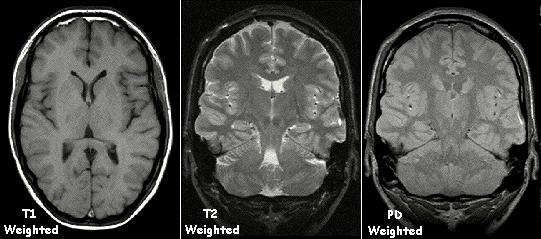
\includegraphics[width=350px]{imagenes/mriscanexample.jpg}
\end{figure}
\begin{figure}[H]
	\label{catscan}
	\caption{Ejemplo de imagen obtenida por CAT}
	\centering
	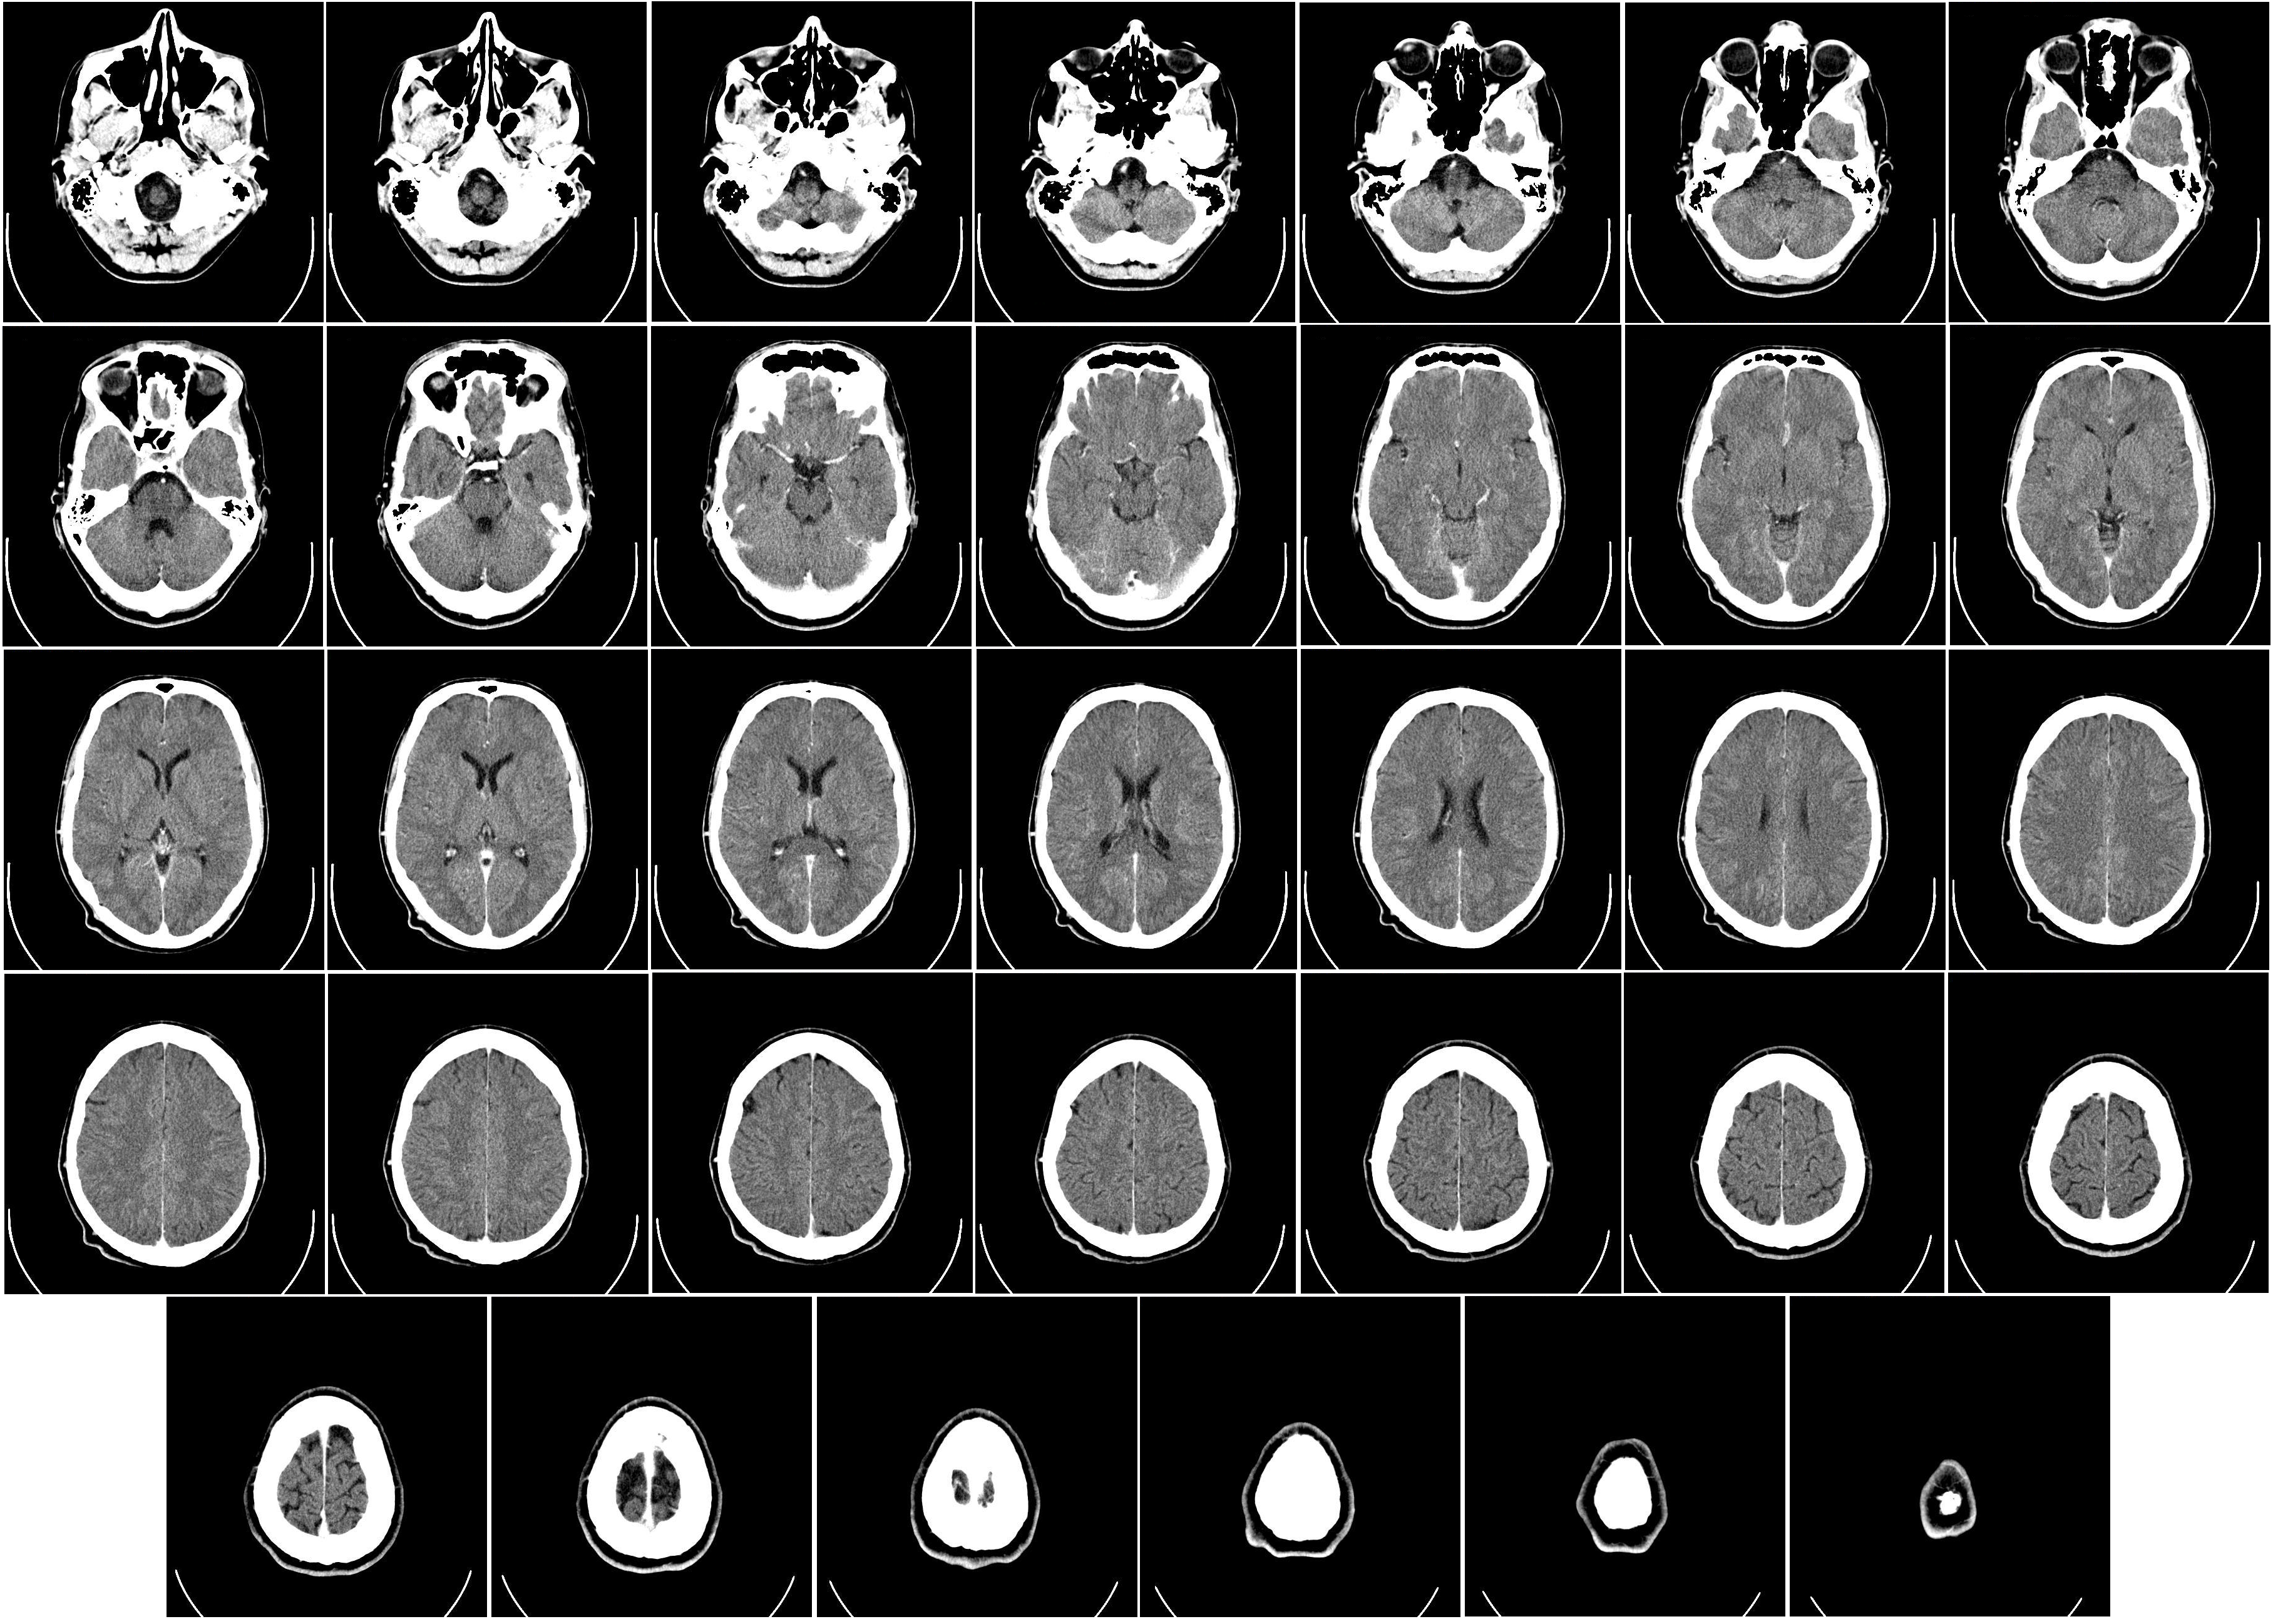
\includegraphics[width=350px]{imagenes/catimage.png}
\end{figure}
\newpage

En la siguiente tomografía del cerebro de un paciente se puede observar la perdida de la función del lóbulo temporal:

\begin{figure}[H]
	\label{perdidaLT}
	\caption{Tomografía del cerebro de un paciente con alzheimer mostrando pérdida de la función en el lóbulo temporal.}
	\centering
	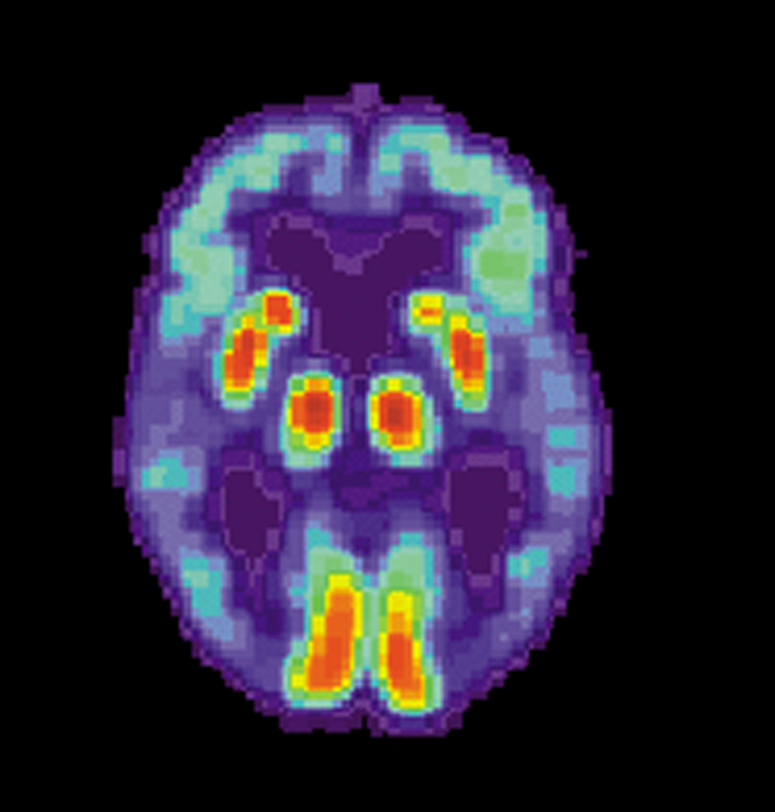
\includegraphics[height=200px,width=200px]{imagenes/perdidaLT.jpg}
\end{figure}


Muchos estudios se han enfocado en cuantificar cuál es la cantidad de atrofia en el lóbulo temporal, e incluso existen escalas para cuantificar cuál es el grado de atrofia, las cuáles son rápidas y fáciles de usar. En la última década, también se han desarrollado métodos automáticos para medir el grado medio de atrofia en el lóbulo temporal \cite{Hattori2007}, y esto se ha utilizado para la predicción de pacientes que padecen la enfermedad \cite{Visser491}.\\

En paralelo, también se ha observado que los pacientes de Alzheimer una notable atrofia en regiones posteriores conocida como atrofia cortical. Esto parece ser característico, pero no exclusivo, de la enfermedad de Alzheimer. Es por ello, que en la última época, se han intentado proponer escalas visuales para cuantificar el grado de atrofia cortical \cite{Koedam2011}.\\

Recientemente también se han realizado estudios sobre la diferencia de la atrofia en el hipocampo y cortical hipo-metabolismo de personas que no padecen la enfermedad y las que sí, pudiendo llevar a mejores diagnósticos. \cite{Chung2017}.\\

También se ha podido observar que la atrofia cerebral comienza años antes del diagnóstico del Alzheimer. De hecho, la atrofia del hipocampo aparece en pacientes con riesgo de padecer Alzheimer años antes de que los síntomas comiencen., como se puede observar en \cite{fox1996presymptomatic}.\\

\section{Análisis de estudios basados en computación}

Por otra parte, el estudio de la enfermedad basándose en el uso del análisis de las imágenes MRI mediante algoritmos de \textit{Machine Learning} es un campo que en la última década ha cobrado mucha fuerza a la hora del diagnóstico de la enfermedad. En \cite{CHAPLOT200686} podemos observar el uso ondas y características de las imágenes para entrenar un algoritmo SVM  y también el uso de redes neuronales con mapas auto organizados de características (SOM) con el fin de clasificar entre cerebros normales o anormales, obteniendo unos buenos resultados de \textit{accuracy}.\\

Estudios siguientes continuaban la misma línea de trabajo, usando como características las ondas cerebrales y luego utilizando algún algoritmo de \textit{Machine Learning} como clasificador. Además, también se incluyeron métodos como el PCA( \textit{Principal Component Analysis}) para reducir el tamaño dimensional de los datos. \cite{Lee:2009:CMF:1697406.1697471}\\

Dentro de nuestra propia universidad, tenemos trabajos que demuestran que el uso de SVM con las apropiadas características de ondas y de las propias imágenes además d el uso del PCA para la reducción de la dimensión, permite obtener unos buenos resultados a la hora de la clasificación, como se puede comprobar en \cite{jaramillo}.\\

Hoy en día, con los avances que se han producido con la introducción de nuevos algoritmos de Deep Learning además del avance en las técnicas de adquisición de imágenes, muchos estudios han intentado utilizar estas técnicas para mejorar la clasificación de los pacientes.\\

La mayoría de estos estudios hacen uso de redes convolucionales con muchas capas para el entrenamiento y aprendizaje de filtros que puedan ser útiles a la hora de clasificar a los pacientes. Entre ellos cabe destacar el siguiente estudio \cite{residualVGG}, en el que se utilizaban imágenes MRI en 3D junto con redes convolucionales tridimensionales para el aprendizaje y clasificación de pacientes. En este se obtienen unos resultados muy destacables, partiendo de una base de datos muy reducida.\\

También se pueden encontrar estudios en los cuáles el uso de redes convolucionales junto con el uso de \textit{autoencoders}, se obtienen buenos resultados en el \textit{accuracy} a la hora de la clasificación de los pacientes, como se puede observar en \cite{DBLP:journals/corr/Hosseini-AslKE16}.\\

Como se puede observar, la mayoría de estudios realizados hacen usos de redes convolucionales en tres dimensiones, lo que produce que se necesite mucha capacidad de computación y tiempo para obtener los resultados del entrenamiento. Este es un campo en el que aún queda mucho desarrollo, sobre todo para llegar a unas técnicas que se pudiesen implantar como ayuda a la toma de decisión de un médico en caso de diagnóstico.\\
